\documentclass[12pt,a4paper]{book}
\usepackage[latin1]{inputenc}
%\usepackage{creativecommons}
\usepackage{xmpincl}
\usepackage{lipsum}
\usepackage{url}
\usepackage{amsmath}
\usepackage{amsfonts}
\usepackage{amssymb}
\usepackage{graphicx}
\usepackage{multicol}
\usepackage[normalem]{ulem} % needed by strike
\usepackage[urlcolor=blue,colorlinks=true,citecolor=blue,linkcolor=black]{hyperref}
\usepackage{makeidx}
\usepackage{color}
\usepackage{xmpincl}
\makeindex
\setcounter{tocdepth}{1}
\author{Paul Sutton}
\begin{document}

\begin{figure}
\centering

\includegraphics[width=0.7\linewidth]{./FinalLogo}

\begin{center}
{\Huge ToriOS Testing Manual}
\end{center}

\end{figure}

\tableofcontents
\index{Table of Contents}

\chapter{Introduction}
This manual is intended to act as a guide to help people test the ToriOS \cite{ToriOS} operating system and give brief overviews in to the different ways that ToriOS can be tested. 

\chapter{Virtual-Box}
\index{Virtualbox}
Text added to make Contents work
\textbf{Part 1 : set up virtual box - GNU / Linux}
To set install Virtual box on Ubuntu you should run the following \\

\begin{itemize}
\item{sudo apt-get install virtualbox-qt}
\item{sudo apt-get install virtualbox-dkms}
\end{itemize} 

After this you need to set up a virtual machine so that the MiniISO can be installed to this.   It is ASSUMED you know how to do this.  However you DO need to enable networking:\\ \\
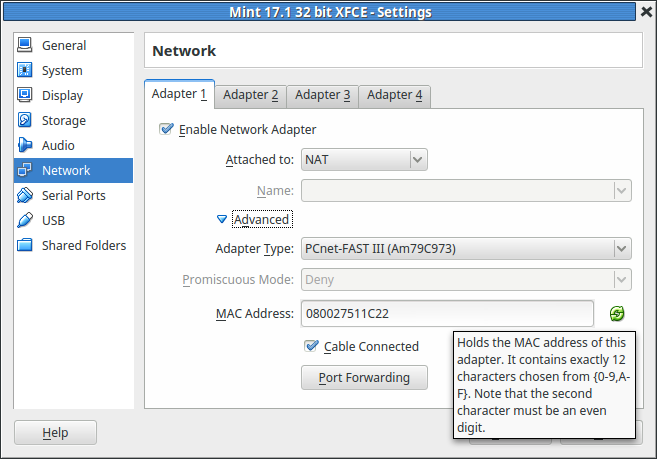
\includegraphics[width=0.7\linewidth]{screen-shots/virtualbox-network} \\

You may also want to check to see if PAE has been enabled as toriOS is designed for NON PAE systems.\\
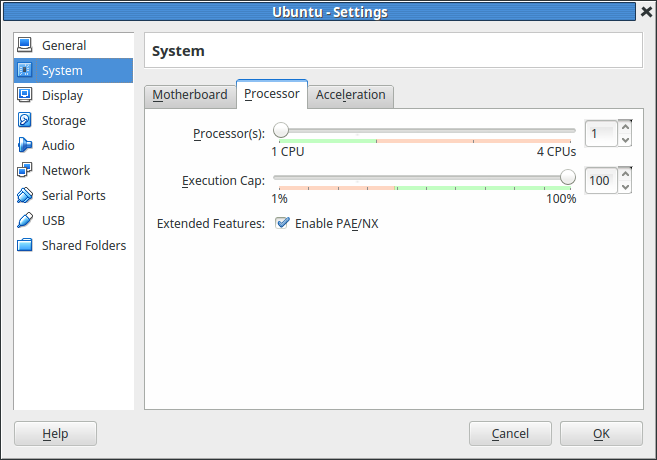
\includegraphics[width=0.7\linewidth]{screen-shots/Virtualbox-enablePAE}


Once done you can run virtual box from the menu.

Components such as USB amd sharing files with the host system are NOT supported unless using virtualbox extensions.  \\



\chapter{Obtaining the Ubuntu Mini ISO}

This step covers what is needed to convert a ubuntu 12.04 mini ISO to use the ToriOS desktop environment and related system components.\\ \\
\textbf{
Step 1:} Install ToriOS into the virtual machine created earlier. 

Download the iso file from the website below \\

http://archive.ubuntu.com/ubuntu/dists/precise-updates/main/installer-i386/current/images/

netboot directory then nonPAE

file mini.iso

You will also need to download the md5sum checksum and verify the download. 

Before you install to this virtual machine you may want to clone it, that way you have a copy for future testing. To do this you need to right click on the virtual machine and select clone,  follow the prompts.   This may take a while but probably works out quicker than keep re-installing the guest OS.


\chapter{Convert mini ISO to ToriOS}

Once you have downloaded and installed the Mini ISO you should be logged in as a default user,  and this user should be a member of the sudo-ers list so you can run sudo (as in run a command as root) as that user. \\
in which case you can wget the shell script and run that to convert to ToriOS\\

Download shell script
wget https://raw.githubusercontent.com/Israel-/torios-from-mini/master/torios-precise-x86.sh

set to execute permissions

chmod +x torios-precise-x86.sh


You can use wget -c for this
\chapter{Install - blank HDD}

This is for a single hard disk install.  This will use the One Button installer \cite{OBI} and will \textbf{WIPE} all data and replace what is on the hard disk with ToriOS. 

\chapter{Install - Multi-Boot} 

This option has 2 steps,  the first is to use gparted \cite{Gparted} to partition your hard disk so that it has space for toriOS and a swap area,  then use OBI to install to that partition.  

\chapter{PDF References}
\index{PDF References}
\label{PDF References}
\begin{center}\begin{tabular}{|l|l|}
\hline \textbf{PDF} & \textbf{Location} \\
\hline Quick start & \htmladdnormallink{mkUSB-quick-start-manual.pdf}{http://phillw.net/isos/linux-tools/mkusb/mkUSB-quick-start-manual.pdf} \\

\hline nox manual & \htmladdnormallink{mkUSB-quick-start-manual-nox.pdf}{http://phillw.net/isos/linux-tools/mkusb/mkUSB-quick-start-manual-nox.pdf} \\

\hline bas manual & \htmladdnormallink{mkUSB-quick-start-manual-bas.pdf}{http://phillw.net/isos/linux-tools/mkusb/mkUSB-quick-start-manual-bas.pdf} \\


\hline Virtual Box User manual & \htmladdnormallink{Virtual Box Manual (HTML) }{http://www.virtualbox.org/manual/UserManual.html}\\

\hline Virtual Box Wiki & \htmladdnormallink{VirtualBox Download}{https://www.virtualbox.org/wiki/VirtualBox}\\

\hline x & \htmladdnormallink{}{}\\

\hline x & \htmladdnormallink{}{}\\

\hline \end{tabular}\end{center}


\begin{thebibliography}{1} % 1 is a random guess of the total number of
%references

\bibitem{ToriOS}
\url{http://www.torios.org}
\emph{2014-15}

\bibitem{Gparted}
\url{http://gparted.org/}

\bibitem{OBI}
\url{https://help.ubuntu.com/community/OBI	}

\bibitem{OBI Quickstart}
\url{https://help.ubuntu.com/community/OBI?action=AttachFile&do=view&target=OBI-quick-start-manual-3.pdf}

\bibitem{VirtualBox}
\url{https://www.virtualbox.org/}

\bibitem{Gparted}
\url{http://gparted.org/}

\end{thebibliography}

\printindex



\end{document}